\documentclass[a4paper, 12pt]{article}
\usepackage[a4paper,top=1.5cm, bottom=1.5cm, left=1cm, right=1cm]{geometry}
\usepackage{cmap}					% поиск в PDF
\usepackage{mathtext} 				% русские буквы в фомулах
\usepackage[T2A]{fontenc}			% кодировка
\usepackage[utf8]{inputenc}			% кодировка исходного текста
\usepackage[english,russian]{babel}	% локализация и переносы

\usepackage{amsmath}
\usepackage{indentfirst}
\usepackage{longtable}
\usepackage{graphicx}
\usepackage{array}

\usepackage{wrapfig}
\usepackage{siunitx} % Required for alignment
\usepackage{subfigure}
\usepackage{multirow}
\usepackage{rotating}
\usepackage{caption}

\graphicspath{{pictures/}}


\title{\begin{center}Лабораторная работа №2.2.6\end{center}
Определение энерги активации по температурной зависимости вязкости жидкости}
\author{Рожков А. В.}
\date{\today}

\begin{document}
    \pagenumbering{gobble}
    \maketitle
    \newpage
    \pagenumbering{arabic}


    \textbf{Цель работы:} измерение скорости падения шариков при разной температуре жидкости; вычисление вязксоти жидкости по закону Стокса и расчет энергии активации.

    \textbf{В работе используются:} стеклянный цилиндр с исследуемой жидкостью (глицерин); термостат; секундомер; горизонтальный компаратор; микроскоп; мелкие шарики (диаметром 1-2 мм).

    \section{Теоретическая часть}
    \subsection{Энергия активации}
    Для того чтобы перейти в новое состояние, молекула жидкости должна преодолеть участки с большой потенциальной энергией, превышающей среднюю тепловую энергию молекул. Для этого тепловая энергия молекул должна — вследствие флуктуации — увеличиться на некоторую величину $W$ , называемую энергией активации. Температурная зависимость вязкости жидкости при достаточно грубых предположениях можно опистаь формулой
    \begin{equation} \label{activation_energy:1}
        \eta \sim A e^{W/kT}
    \end{equation}

    Из формулы (\ref{activation_energy:1}) следует, что существует линейня зависимость между величинами $ln\eta$ и $1/T$, и энергию активации можно найти по формуле

    \begin{equation} \label{activation_energy:2}
        W = k \frac{d(ln\eta)}{d(1/T)}
    \end{equation}

    \subsection{Измерение вязкости}
    По формуле Стокса, если шарик радиусом $r$ и со скоростью $v$ движется в среде с вязкостью $\eta$, и при этом не наблюдается турбулентных явлении, тормозящую силу можно найти по формуле (\ref{stokes})

    \begin{equation}\label{stokes}
        F = 6\pi\eta \frac{d}{2}v
    \end{equation}


    Для измерения вязкости жидкости рассмотрим свободное падение шарика в жидкости. При медленных скоростях на шарик действуют силы Архимеда и Стокса, выражения для которых мы знаем. Отсюда находим выражения для установившейся скорости шарика и вязкости жидкости

    \begin{align}
        v_{уст}&=\frac{2}{9}g\frac{d^2}{4}\frac{\rho - \rho_ж}{\eta}\label{v_ust}\\
        \eta&=\frac{2}{9}g\frac{d^2}{4}\frac{\rho - \rho_ж}{v_{уст}}\label{eta}
    \end{align}

    Как видим, измерив установившуюся скорость шарика и параметры системы можно получить вязкость по формуле (\ref{eta}).

    \subsection{Экспериментальная установка}
    Для измерений используется стеклянный цилиндрчиеский сосуд B, наполненный исследуемой жидкостью (глицерин). Диаметр сосуда $\approx 3$ см, длина $\approx 25$ см. На стенках сосуда нанесены две метки на некотором расстоянии друг от друга. Верхняя метка должна располагаться ниже уровня жидкости с таким расчетом, чтобы скорость шарика к моменту прохождения этой метки успевала установиться. Измеряя расстояние между метками, b время падения определяют установившуюся скорость шарика $v_{уст}$. Сам сосуд B помещен в рубашку D, омываемую водой из термостата. При работающем термостате температура воды в рубашке D, а потому и температура жидкости 12 равна температуре воды в термостате.
    Схема прибора (в разрезе) показана на рис.~\ref{ustanovka}.
    \begin{figure}[ht]
        \center{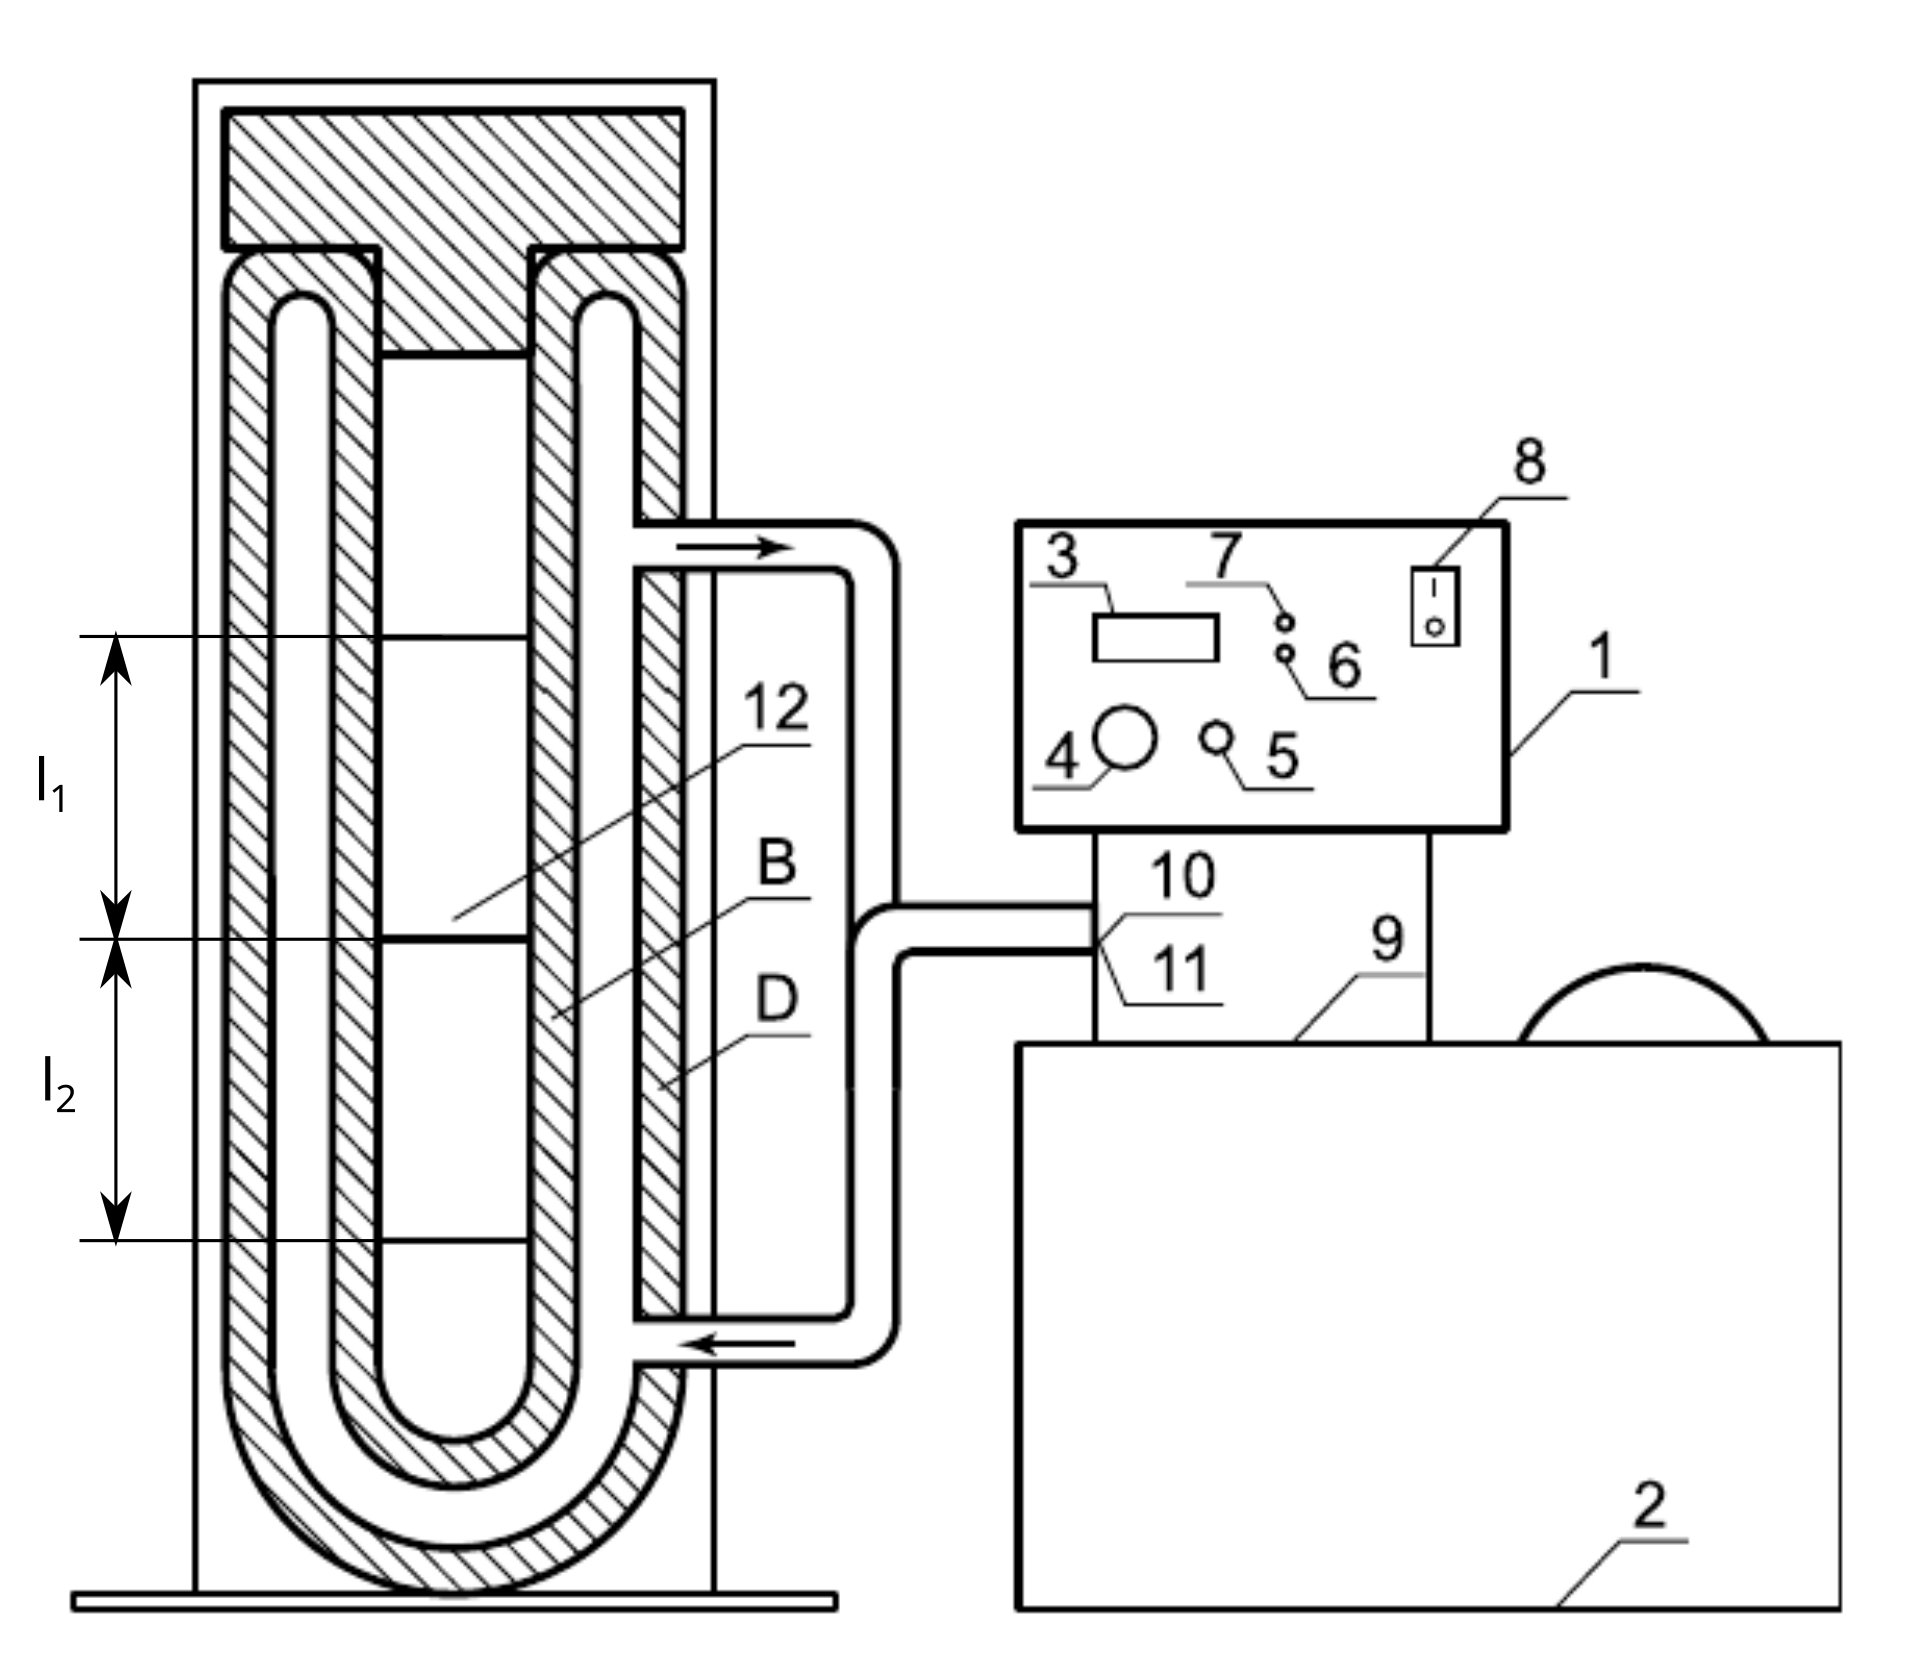
\includegraphics[scale=0.5]{ustanovka}}
        \caption{Установка для определения коэффициента вязкости жидкости.}
        \label{ustanovka}
    \end{figure}

    \section{Ход работы}
    \subsection{Измерение диаметра шариков}

    Выбираем 12 стальных и 12 стеклянных шариков. Из-за неидеальности формы измерения производим в 2 случайных направлениях при помощи микроскопа и усредняем. Данные измерений приведены в таблице~\ref{diameters}. Погрешность измерений $\sigma_d = 0.02~мм$. Плотности шариков:

    \begin{align*}
        \rho_{стекло}&=2.5~г/см^3\\
        \rho_{сталь}&=7.8~г/см^3
    \end{align*}

    \begin{table}[!ht]
        \centering
        \subtable{
            \begin{tabular}{|c|c|c|}
            \hline
                № & Материал & Диаметр, мм \\ \hline
                1 & Стекло & 2,07 \\ \hline
                2 & Стекло & 2,08 \\ \hline
                5 & Стекло & 2,11 \\ \hline
                6 & Стекло & 2,1 \\ \hline
                9 & Стекло & 2,09 \\ \hline
                11 & Стекло & 2,12 \\ \hline
                13 & Стекло & 2,09 \\ \hline
                14 & Стекло & 2,12 \\ \hline
                17 & Стекло & 2,09 \\ \hline
                18 & Стекло & 2,12 \\ \hline
                21 & Стекло & 2,12 \\ \hline
                22 & Стекло & 2,16 \\ \hline
            \end{tabular}
        }
        \subtable{
            \begin{tabular}{|c|c|c|}
            \hline
                № & Материал & Диаметр, мм \\ \hline
                3 & Сталь & 0,85 \\ \hline
                4 & Сталь & 0,75 \\ \hline
                7 & Сталь & 0,81 \\ \hline
                8 & Сталь & 0,72 \\ \hline
                10 & Сталь & 0,71 \\ \hline
                12 & Сталь & 0,84 \\ \hline
                15 & Сталь & 0,78 \\ \hline
                16 & Сталь & 0,91 \\ \hline
                19 & Сталь & 0,83 \\ \hline
                20 & Сталь & 0,91 \\ \hline
                23 & Сталь & 0,78 \\ \hline
                24 & Сталь & 0,79 \\ \hline
            \end{tabular}
        }
        \caption{Измеренные диаметры шариков}
        \label{diameters}
    \end{table}

    \subsection{Измерение установившихся скоростей падения шариков}

    Измеренные длины частей цилиндра установки (см. рис.~\ref{ustanovka}):

    \begin{align*}
        l_1 = l_2 = (10 \pm 0.1)~см
    \end{align*}

    Измерения производим для 6 значений температуры от 25 до 50 $ ^\circ C $. При помощи секундомера измеряем время прохождения шариком участков $l_1$ и $l_2$. Усредняем значение, вычислеям установившуюся скорость шариков в жидкости. По графику на рис.~\ref{density} определим плотность глицерина для каждой температуры. По формуле~(\ref{eta}) рассчитываем вязкость глицерина. Результаты представлены в таблице~\ref{velocities}.

    \begin{figure}[ht]
        \center{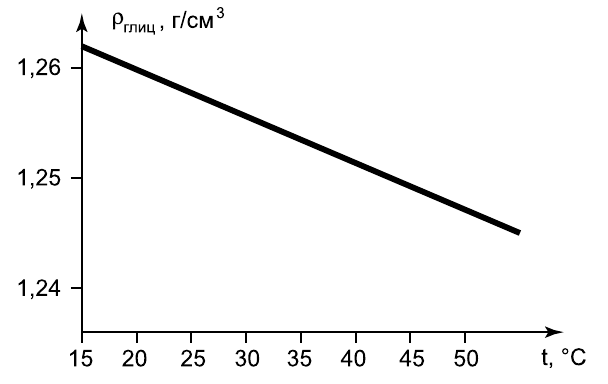
\includegraphics[scale=0.5]{density.png}}
        \caption{График плотности глицерина в зависимости от температуры.}
        \label{density}
    \end{figure}

    \begin{table}[!ht]
        \centering
        \begin{tabular}{|c|c|c|c|c|c|c|c|c|}
        \hline
            № & Материал & $T, K$ & $t_{l_1}, с$& $t_{l_1}, с$ & $t_{ср}, с$ & $v_{уст}, мм/c$ & $\rho_глиц, г/см^3$ & $\eta, мПа * с$  \\ \hline
            1 & Стекло & 298 & 27,9 & 27,85 & 27,875 & 3,587443946 & 1,258  & 808  \\ \hline
            2 & Стекло & 298 & 27,26 & 27,06 & 27,16 & 3,681885125 & 1,258  & 795  \\ \hline
            3 & Сталь & 298 & 29,08 & 29 & 29,04 & 3,443526171 & 1,258  & 747  \\ \hline
            4 & Сталь & 298 & 34,83 & 34,51 & 34,67 & 2,884338044 & 1,258  & 695  \\ \hline
            5 & Стекло & 303 & 18,76 & 18,87 & 18,815 & 5,314908318 & 1,256  & 568  \\ \hline
            6 & Стекло & 303 & 18,56 & 18,67 & 18,615 & 5,372011818 & 1,256  & 556  \\ \hline
            7 & Сталь & 303 & 21,89 & 21,85 & 21,87 & 4,572473708 & 1,256  & 511  \\ \hline
            8 & Сталь & 303 & 26,6 & 26,64 & 26,62 & 3,756574005 & 1,256  & 492  \\ \hline
            9 & Стекло & 308 & 12,64 & 12,71 & 12,675 & 7,889546351 & 1,253  & 376  \\ \hline
            10 & Сталь & 308 & 17,64 & 18,14 & 17,89 & 5,589714925 & 1,253  & 321  \\ \hline
            11 & Стекло & 308 & 12,21 & 12,08 & 12,145 & 8,233841087 & 1,253  & 370  \\ \hline
            12 & Сталь & 308 & 14,82 & 15,19 & 15,005 & 6,664445185 & 1,253  & 377  \\ \hline
            13 & Стекло & 313 & 8,64 & 8,53 & 8,585 & 11,64822365 & 1,251  & 255  \\ \hline
            14 & Стекло & 313 & 8,4 & 8,38 & 8,39 & 11,91895113 & 1,251  & 256  \\ \hline
            15 & Сталь & 313 & 10,83 & 10,97 & 10,9 & 9,174311927 & 1,251  & 236  \\ \hline
            16 & Сталь & 313 & 8,4 & 8,23 & 8,315 & 12,02645821 & 1,251  & 246  \\ \hline
            17 & Стекло & 318 & 6,67 & 6,42 & 6,545 & 15,27883881 & 1,249  & 195  \\ \hline
            18 & Стекло & 318 & 6,4 & 6,49 & 6,445 & 15,5159038 & 1,249  & 197  \\ \hline
            19 & Сталь & 318 & 8,07 & 8,13 & 8,1 & 12,34567901 & 1,249  & 199  \\ \hline
            20 & Сталь & 318 & 7,03 & 6,77 & 6,9 & 14,49275362 & 1,249  & 204  \\ \hline
            21 & Стекло & 323 & 4,8 & 4,81 & 4,805 & 20,81165453 & 1,247  & 147  \\ \hline
            22 & Стекло & 323 & 4,86 & 4,61 & 4,735 & 21,11932418 & 1,247  & 151  \\ \hline
            23 & Сталь & 323 & 5,53 & 5,58 & 5,555 & 18,00180018 & 1,247  & 121  \\ \hline
            24 & Сталь & 323 & 5,67 & 5,75 & 5,71 & 17,51313485 & 1,247  & 127  \\ \hline
        \end{tabular}
        \caption{Результаты измерений установившившихся скоростей шариков и соответствующих плотностей глицерина}
        \label{velocities}
    \end{table}

    \subsection{Вычисление числа Рейнольдса, оцена времени и пути релаксации. Анализ применимости формулы Стокса}

    Для каждого из опытов вычислим число Рейнольдса $Re$~(\ref{Re}), оценим время релаксации $\tau$~(\ref{relax_time}) и путь релаксации $S$~(\ref{S}). Результаты представлены в таблице~\ref{re_tau_s}.

    \begin{align}
        Re &= \frac{d}{2} \frac{v_{уст} \rho_{глиц}}{\eta} \label{Re}\\
        \tau &= \frac{2}{9} \frac{d^2}{4} \frac{\rho}{\eta} \label{relax_time}\\
        S &= v_{уст} \tau \label{S}
    \end{align}

    \begin{table}[!ht]
        \centering
        \begin{tabular}{|c|c|c|c|c|c|c|}
            \hline
            № & материал & $T, K$ & $\eta, мПа * с$ & $Re$ & $\tau, мс$ & $S, мкм$ \\ \hline
            1 & Стекло & 298 & 808 & 0,006 & 0,74 & 2,64  \\ \hline
            2 & Стекло & 298 & 795 & 0,006 & 0,76 & 2,78  \\ \hline
            3 & Сталь & 298 & 747 & 0,002 & 0,42 & 1,44  \\ \hline
            4 & Сталь & 298 & 695 & 0,002 & 0,35 & 1,01  \\ \hline
            5 & Стекло & 303 & 568 & 0,012 & 1,09 & 5,79  \\ \hline
            6 & Стекло & 303 & 556 & 0,013 & 1,10 & 5,92  \\ \hline
            7 & Сталь & 303 & 511 & 0,005 & 0,56 & 2,54  \\ \hline
            8 & Сталь & 303 & 492 & 0,003 & 0,46 & 1,72  \\ \hline
            9 & Стекло & 308 & 376 & 0,027 & 1,61 & 12,74  \\ \hline
            10 & Сталь & 308 & 321 & 0,008 & 0,68 & 3,80  \\ \hline
            11 & Стекло & 308 & 370 & 0,030 & 1,68 & 13,87  \\ \hline
            12 & Сталь & 308 & 377 & 0,009 & 0,81 & 5,40  \\ \hline
            13 & Стекло & 313 & 255 & 0,060 & 2,38 & 27,71  \\ \hline
            14 & Стекло & 313 & 256 & 0,062 & 2,43 & 29,02  \\ \hline
            15 & Сталь & 313 & 236 & 0,019 & 1,11 & 10,23  \\ \hline
            16 & Сталь & 313 & 246 & 0,028 & 1,46 & 17,58  \\ \hline
            17 & Стекло & 318 & 195 & 0,102 & 3,12 & 47,60  \\ \hline
            18 & Стекло & 318 & 197 & 0,104 & 3,16 & 49,09  \\ \hline
            19 & Сталь & 318 & 199 & 0,032 & 1,50 & 18,52  \\ \hline
            20 & Сталь & 318 & 204 & 0,040 & 1,76 & 25,52  \\ \hline
            21 & Стекло & 323 & 147 & 0,187 & 4,24 & 88,16  \\ \hline
            22 & Стекло & 323 & 151 & 0,189 & 4,30 & 90,78  \\ \hline
            23 & Сталь & 323 & 121 & 0,073 & 2,19 & 39,36  \\ \hline
            24 & Сталь & 323 & 127 & 0,068 & 2,13 & 37,25  \\ \hline
        \end{tabular}
        \caption{Результаты вычисления $Re$, $\tau$, $S$}
        \label{re_tau_s}
    \end{table}

    Как видим, во всех экспериментах число Рейнольдса меньше 1, а путь релаксации пренебрежимо мал. Следовательно формула Стокса применима.

    \subsection{График зависимости $ln \eta$ от $1/T$}

    \begin{figure}[ht]
        \center{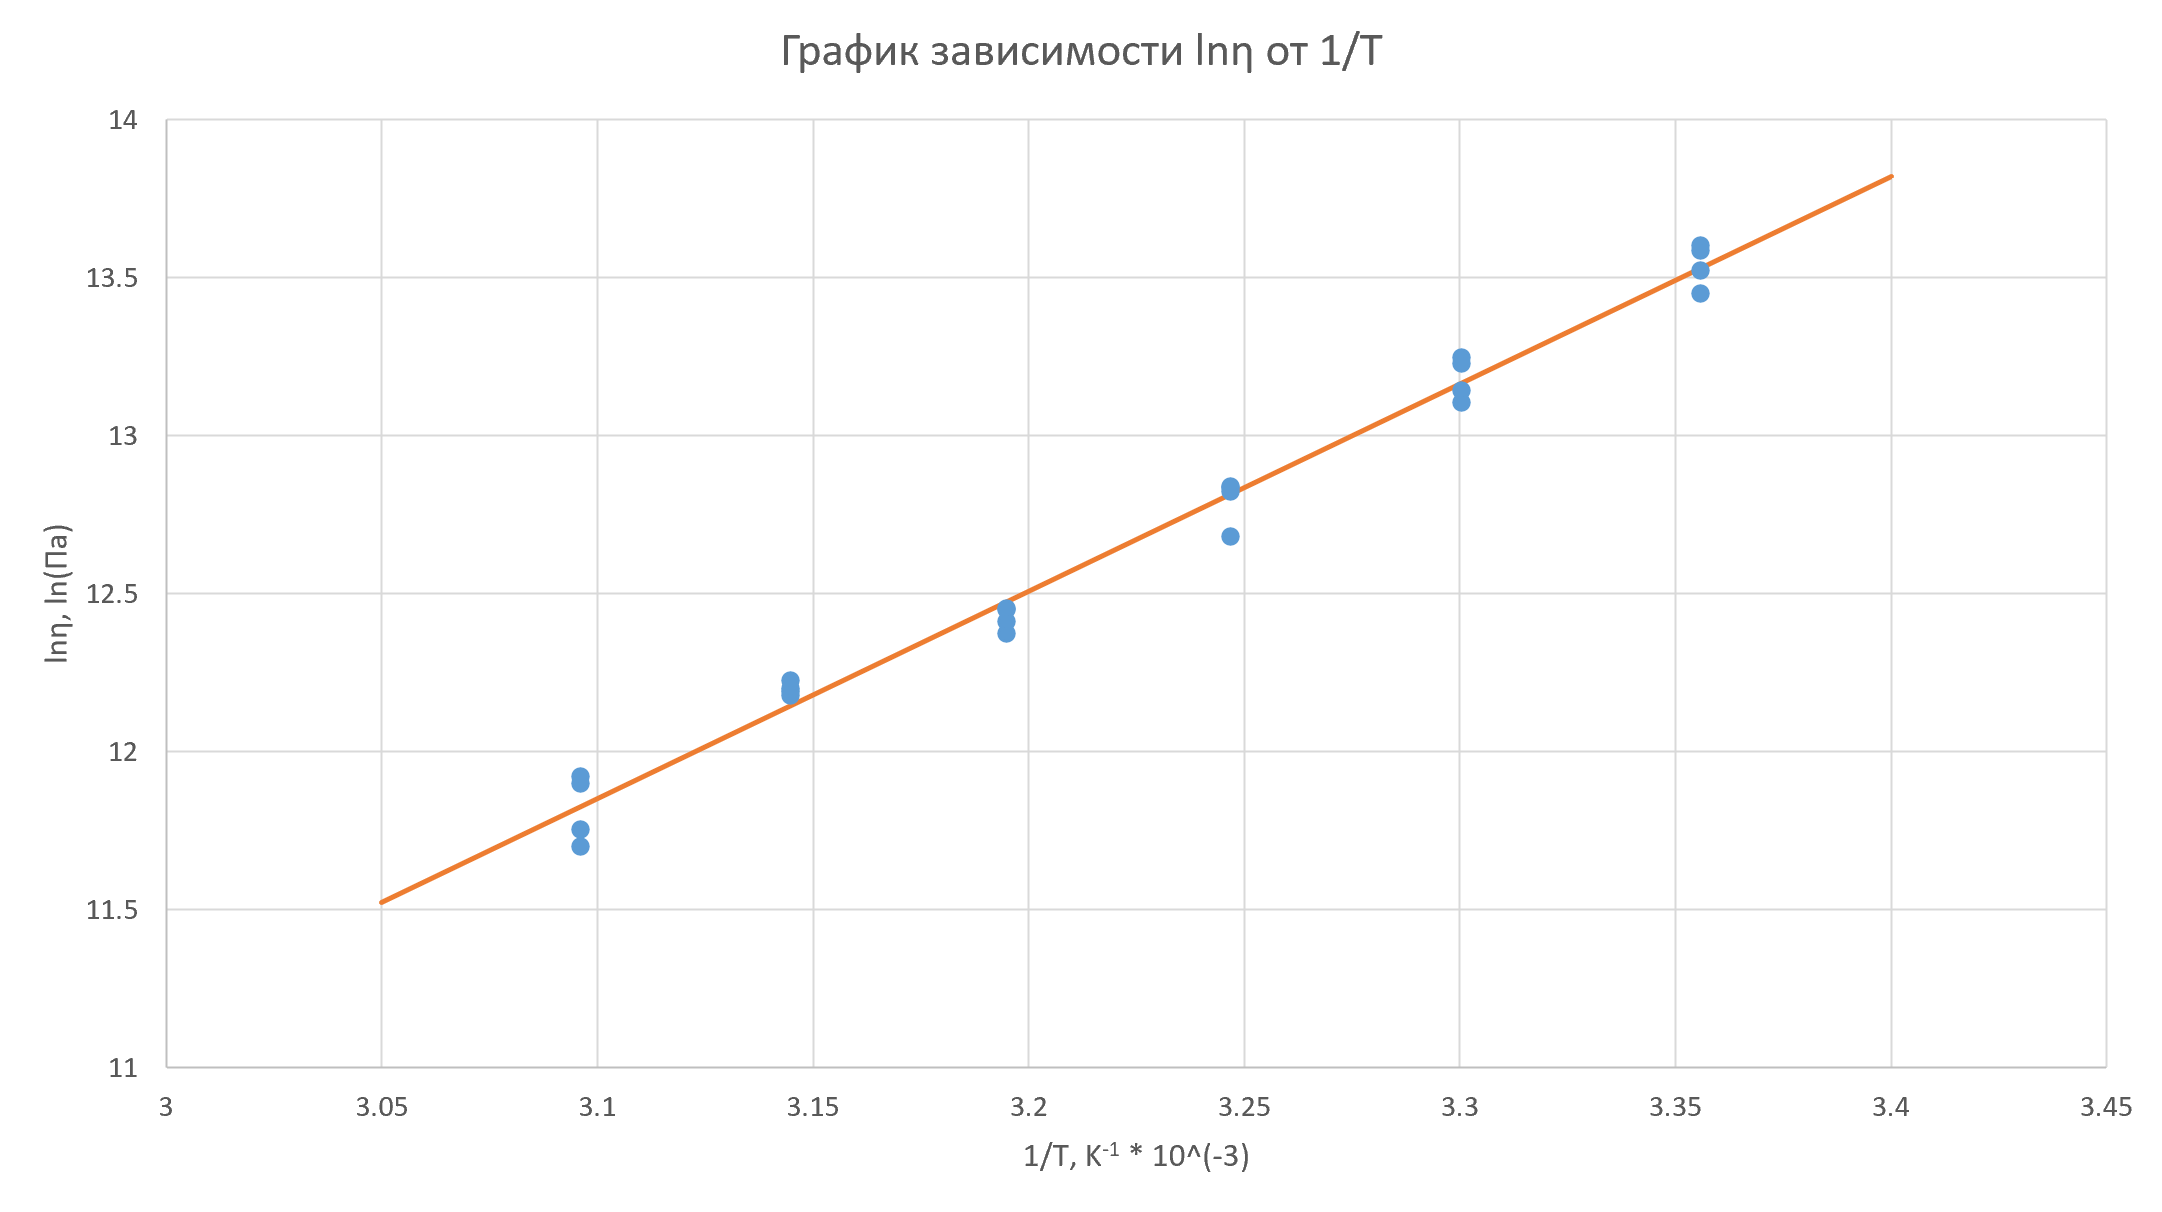
\includegraphics[scale=0.8]{graph.png}}
        \caption{График зависимости $ln \eta$ от $1/T$.}
        \label{graph}
    \end{figure}

    По методу наименьших квадратов вычислим угол наклона прямой.

    \begin{align*}
        k_{накл} = \frac{\langle xy \rangle - \langle x \rangle \langle y \rangle}{\langle x^2 \rangle - \langle x \rangle^2} = (6570 \pm 160) К
    \end{align*}

    Прямая, полученная по МНК не проходит через 0. Это объясняется тем, что в формуле (\ref{activation_energy:1}) есть константа $A$. Коэффициент $b$ прямой соответсвенно равен $lnA$.

    \subsection{Вычисление энергии активации}

    При помощи формулы (\ref{activation_energy:2}) рассчитаем энергию активации:

    \begin{align*}
        W = k * k_{накл} = 1.38 * 10^{-23} Дж/К * 6570~К = 90.66~зДж
    \end{align*}

    \subsection{Оценка погрешностей}

    Случайная погрешность коэффициента наклона прямой:

    \begin{align*}
        \sigma_{k_{накл}} = \frac{1}{\sqrt{24}} \sqrt{\frac{\langle y^2 \rangle - {\langle y \rangle}^2}{\langle x^2 \rangle - {\langle x \rangle}^2} - k_{накл}^2} = 160~K
    \end{align*}

    Полная погрешность энергии активации:

    \begin{align*}
        \sigma_{W} = k * \sigma_{k_{накл}} = 1.38 * 10^{-23} Дж/К * 160 K = 2~зДж
    \end{align*}

    \section{Вывод}

    \begin{align*}
        W = (91 \pm 2)~зДж
    \end{align*}

    Измерили скорости падения шариков при разной температуре жидкости, вычислили вязкость жидкости по закону Стокса и рассчитали энергию активации. Полученная вязкость глицерина при $25^\circ C$ совпадает с табличным значением.

\end{document}
